\section*{Lezione 8}
\addcontentsline{toc}{section}{Lezione 8}

Portando le probabilità virtuali uguali sopra quindi abbiamo detto si ridurrà la varianza (scelta che preferiamo per robustezza ecc).
\medskip

\textbf{Es.4.8-2 pag.68}
Creare codice ottimale per le seguenti probabilità:\\
\begin{equation*}
\frac{1}{3} \; \; | \; \;
\frac{1}{4} \; \; | \; \;
\frac{1}{5} \; \; | \; \;
\frac{1}{6} \; \; | \; \;
\frac{1}{20}
\end{equation*}


\begin{figure}[h]
	\centering
	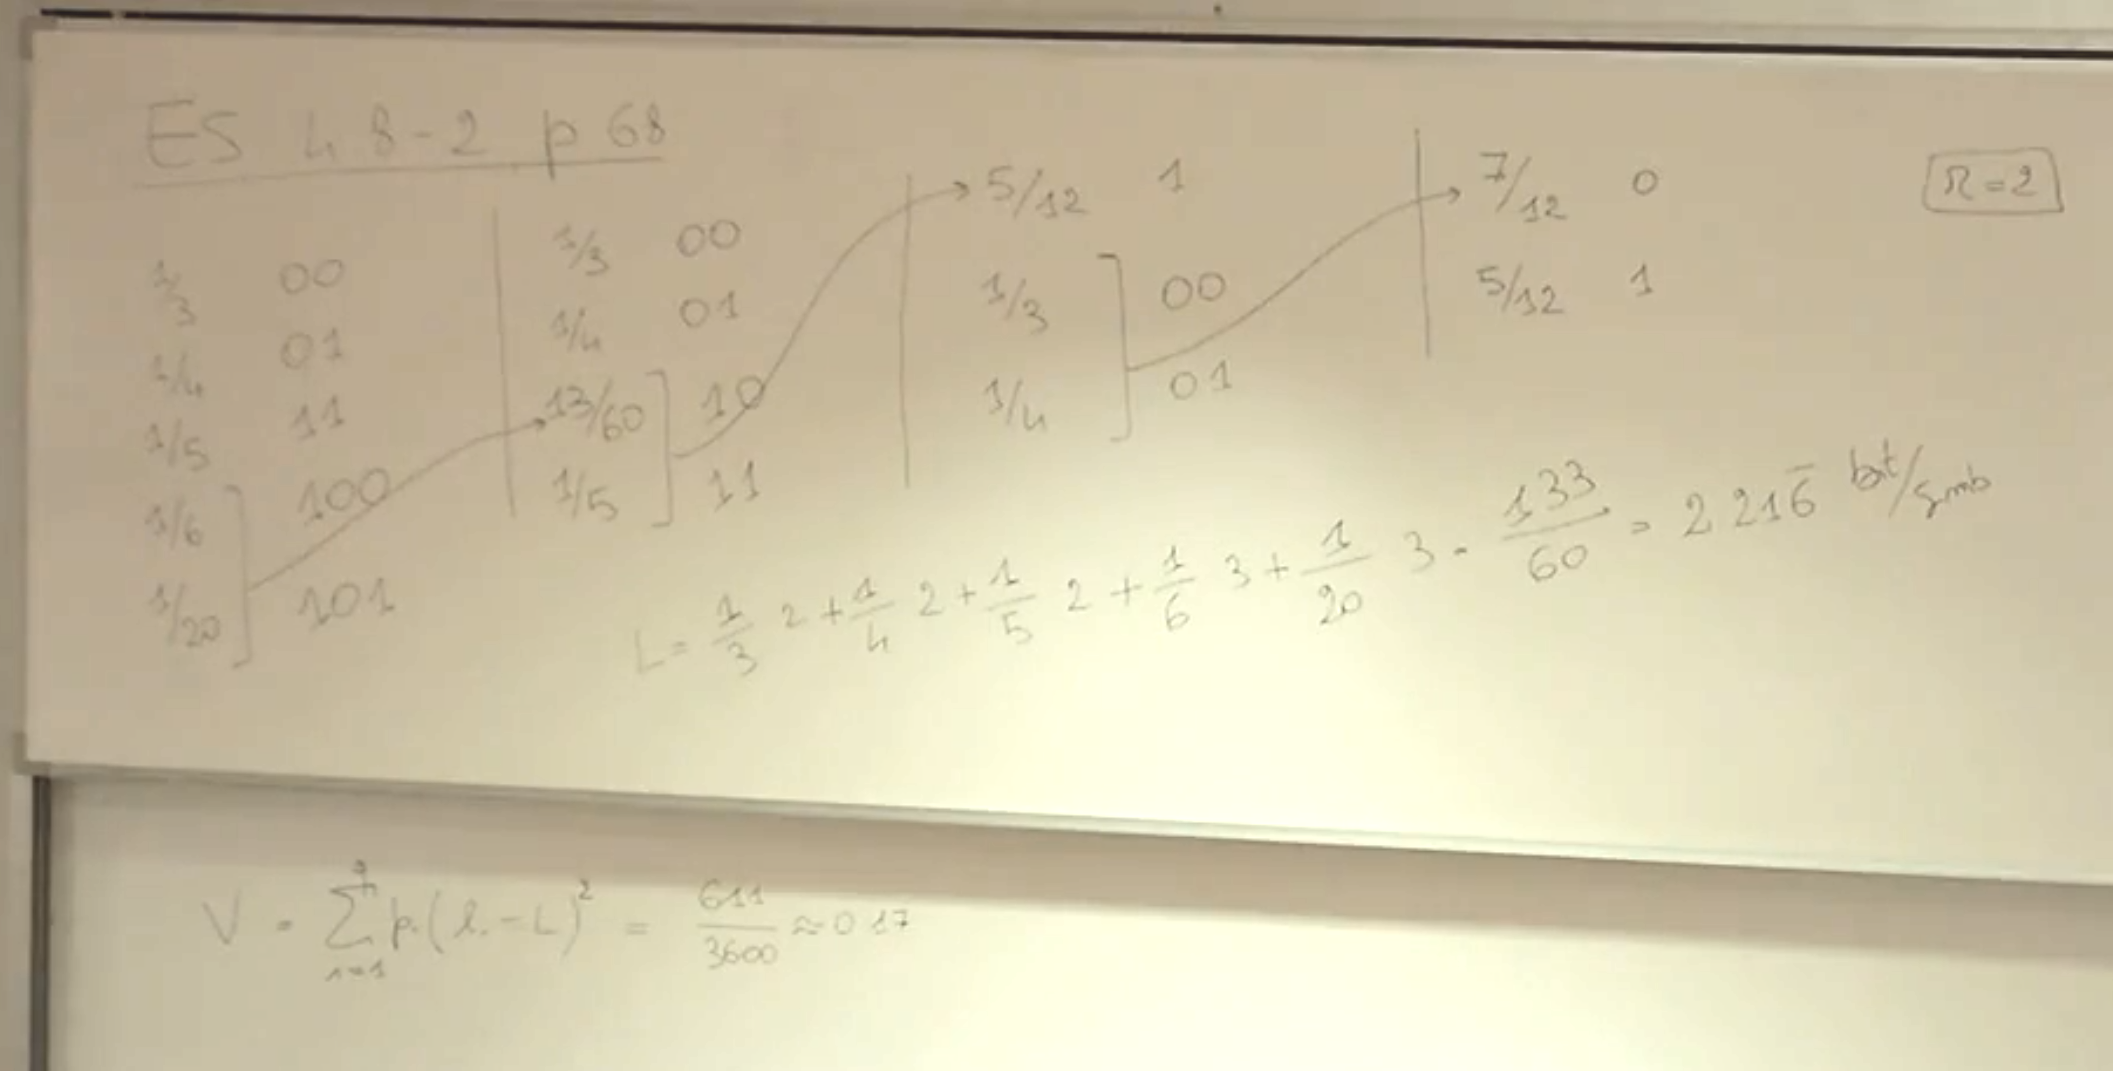
\includegraphics[width=\linewidth]{immagini/img18}
\end{figure}

Non è possibile costruire codice binario istantaneo migliore (in termini di lunghezza media) di quello prodotto dall'algoritmo di Huffman

\begin{dimostrazione}
	Per assurdo:\\
	Consideriamo delle probabilità $p_1, p_2, ... , p_q$ e una $L$ dell'algoritmo di Huffman. Succcessiamente consideriamo una $L'$ ipoteticamente migliore, quindi diciamo che $L'<L$.
	Consideriamo l'albero i due alberi costruiti:
	\begin{multicols}{2}
		Albero algoritmo Huffman:\\
		\begin{center} $L$ \end{center}
		\begin{Figure}
			\centering
			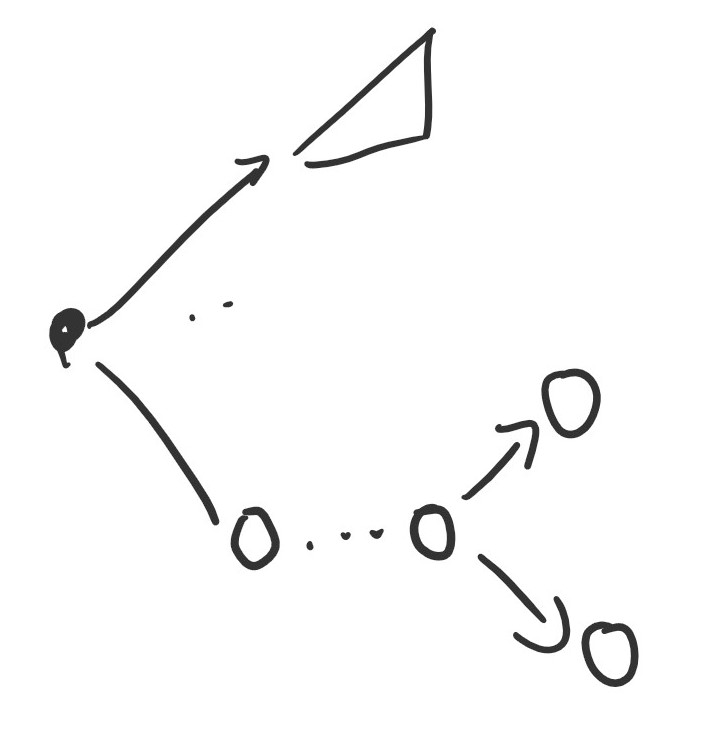
\includegraphics[width=0.7\linewidth]{immagini/img19}
		\end{Figure}
		
		\columnbreak
		
		Albero algoritmo "migliore":\\
	    \begin{center}	$L'<L$ \end{center}
		\begin{Figure}
			\centering
			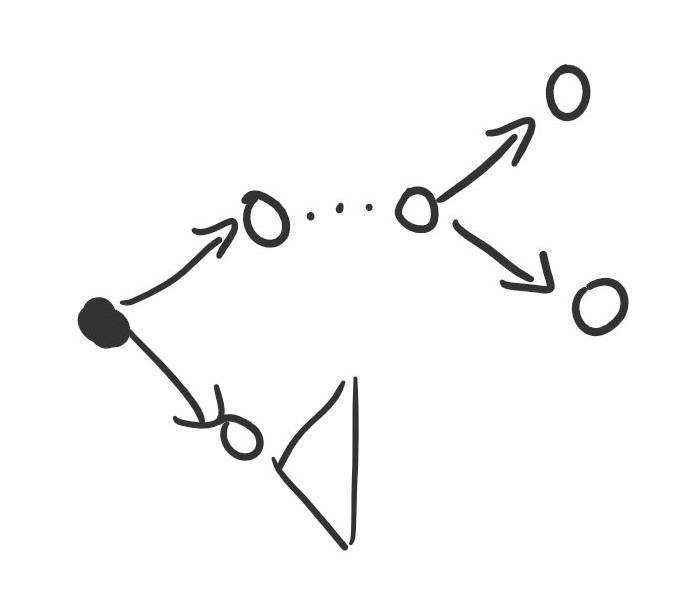
\includegraphics[width=0.7\linewidth]{immagini/img20}
		\end{Figure}
	\end{multicols}

	Ora soffermiamoci sui due codici più lunghi. Ricordiamo che in un codice ottimale, le probabilità sono ordinate in modo decrescente e le lunghezze in modo crescente. In altri termini:
	
	\begin{equation*}
	p_1 \geq p_2 \geq ... \geq p_{q-1} \geq p_q
	\end{equation*}
		\begin{equation*}
	\ell_1 \leq \ell_2 \leq ... \leq \ell_{q-1} \leq \ell_q
	\end{equation*}
	
	Ricordiamoci che le ultime due codeword in ordine di lunghezza devono essere uguali (pensa all'albero, se non sono uguali vuol dire che ho un nodo di decisione con un solo figlio), quindi:
	\begin{equation*}
	\ell_{q-1} = \ell_{q}
	\end{equation*}
	

	
	Nel calcolo di $L$ avrò che negli ultimi due termini andrò a sommare\\ $(\ell_{q-1} \cdot p_{q-1}) + (\ell_q \cdot p_q)$, ma visto che $\ell_{q-1} = \ell_{q}$ è come se stessi facendo
	\begin{equation*}
	\ell_q(p_{q-1} + p_q)
	\end{equation*}
	
		Soffermiamoci su questi due caratteri e consideriamo l'ultimo sottoalbero; sostituiamolo con un singolo nodo "virtuale" (come accade nell algoritmo di huffman):
	\begin{figure}[h]
		\centering
		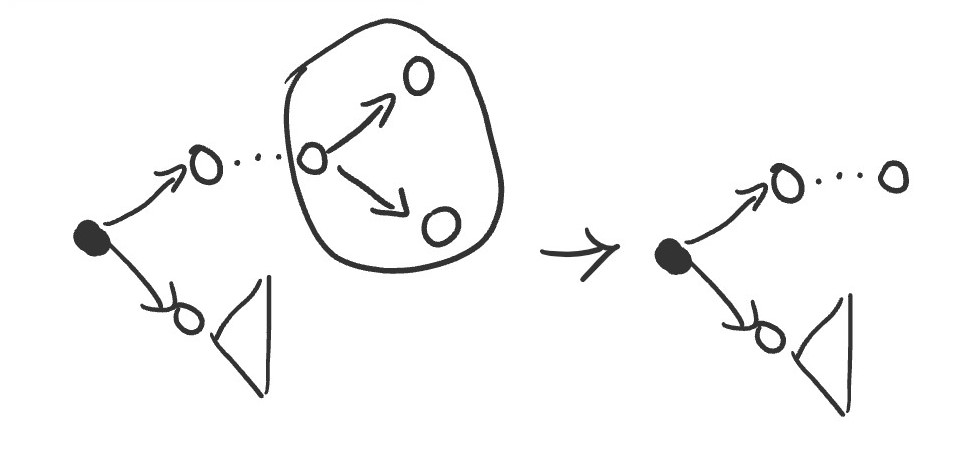
\includegraphics[width=0.7\linewidth]{immagini/img21}
	\end{figure}

	Avendo effettuato questa operazione, nella lunghezza media il contributo diventa:
	\begin{equation*}
	\ell_q - 1(p_{q-1} + p_q)
	\end{equation*}
	\begin{center}
		\footnotesize N.B. sottraggo uno in quando scendo di un livello nell'albero, quindi le codeword avranno un carattere in meno
		\normalsize
	\end{center}
	Questa operazione accorcia le lunghezze medie dei due algoritmi in maniera uguale.
	A questo punto avrò un albero che rappresenta una sorgente di $q-1$ simboli.
	Continuo iterativamente ad accorciare gli alberi risultanti, facendo ridurre la lunghezza media in modo uguale nei due algoritmi.
	Alla fine per Huffman arriverò all'albero con due soli simboli, la cui lunghezza media è 1, a questo punto l'altro algoritmo dovrebbe avere un'albero con lunghezza media di lunghezza $<1$, ma che non ha senso!
	
	\begin{multicols}{2}

	\begin{figure}[H]
		\centering
		\caption*{\small{Albero minimale di Huffman con $L = 1$}}
		\begin{tikzpicture}
		[
		grow                    = right,
		level 1/.style={sibling distance=8em},
		level 2/.style={sibling distance=5em},
		level distance          = 5em,
		edge from parent/.style = {draw, -latex},
		every node/.style       = {font=\footnotesize},
		sloped
		]
		\node [root] {}
		child { node [dummy] {}
			edge from parent node [below] {1}}
		child { node [dummy] {}
			edge from parent node [above] {0}}
		;
		\end{tikzpicture}
	\end{figure}

	\small{Albero minimale dell'algoritmo migliore con $L<1$}
\begin{center}
		\Huge{?}
\end{center}	



	\end{multicols}

Quindi l'esistenza di tale algoritmo è assurda
\end{dimostrazione}

\subsection*{Algoritmo di Huffman con $r>2$}
\addcontentsline{toc}{subsection}{Huffman con $r>2$}

Ora proviamo a lavorare con $r=3$, con cifre 0, 1, 2.

Supponiamo di avere una sorgente di quattro simboli con probabilità:
\begin{center}
	$p_1 = 0.4$\\
	$p_2 = 0.3$\\
	$p_3 = 0.2$\\
	$p_4 = 0.1$
\end{center}

A questo punto lanciamo l'algoritmo di Huffman:


\begin{multicols}{2}
	\begin{center}
			$p_1 = 0.4 \rightarrow \texttt{1}$\\
			$p_2 = 0.3 \rightarrow \texttt{00}$\\
			$p_3 = 0.2 \rightarrow \texttt{01}$\\
			$p_4 = 0.1 \rightarrow \texttt{02}$\\
		\end{center}
		
		\columnbreak
		
		\begin{center}
			$p_{2,3,4} = 0.6 \rightarrow \texttt{0}$\\
			$p_1 = 0.4 \rightarrow \texttt{1}$\\

		\end{center}  		
\end{multicols}


\begin{figure}[H]
	\centering
	\vspace{4mm}
	\begin{tikzpicture}
	[
	grow                    = right,
	level 1/.style={sibling distance=8em},
	level 2/.style={sibling distance=5em},
	level distance          = 7em,
	edge from parent/.style = {draw, -latex},
	every node/.style       = {font=\footnotesize},
	sloped
	]
	\node [root] {}
	child { node [dummy] {$s_1$}
		edge from parent node [above] {1}}
	child { node [dummy] {}
		child { node [dummy] {$s_4$}
			edge from parent node [above] {2}}
		child { node [dummy] {$s_3$}
			edge from parent node [above] {1}}
			child { node [dummy] {$s_2$}
			edge from parent node [above] {0}}
		edge from parent node [above] {0}}
	;
	\end{tikzpicture}
\end{figure}
\begin{equation*}
L=1 \cdot 0.4 + 2 \cdot (0.3+0.2+0.1)=1.6\;\frac{\text{cifre ternarie}}{\text{simbolo}}
\end{equation*}

Però questo albero non è ottimale! Lo si può correggere in questo modo:

\begin{figure}[H]
	\centering
	\vspace{4mm}
	\begin{tikzpicture}
	[
	grow                    = right,
	level 1/.style={sibling distance=5em},
	level 2/.style={sibling distance=5em},
	level distance          = 7em,
	edge from parent/.style = {draw, -latex},
	every node/.style       = {font=\footnotesize},
	sloped
	]
	\node [root] {}
	child { node [dummy] {$s_4$}
		edge from parent node [above] {2}}
	child { node [dummy] {$s_1$}
		edge from parent node [above] {1}}
	child { node [dummy] {}
		child { node [dummy] {$s_3$}
			edge from parent node [above] {1}}
		child { node [dummy] {$s_2$}
			edge from parent node [above] {0}}
		edge from parent node [above] {0}}
	
	;
	\end{tikzpicture}
\end{figure}
\begin{equation*}
L=1 \cdot (0.4+0.1) + 2 \cdot (0.3+0.2)=1.5\;\frac{\text{cifre ternarie}}{\text{simbolo}}
\end{equation*}

C'è qualche problema quindi con l'algoritmo applicato ad un $r \neq 2$.In particolare vorrei che dalla radice uscissero tutti i simboli di gamma.

Nell'esempio precedente, potrei lavorare in questo modo:

\begin{multicols}{2}
	\begin{center}
		$p_1 = 0.4 \rightarrow \texttt{0}$\\
		$p_2 = 0.3 \rightarrow \texttt{2}$\\
		$p_3 = 0.2 \rightarrow \texttt{10}$\\
		$p_4 = 0.1 \rightarrow \texttt{11}$\\
	\end{center}
	
	\columnbreak
	
	\begin{center}
		$p_1 = 0.4 \rightarrow \texttt{0}$\\
		$p_{3,4} = 0.3 \rightarrow \texttt{1}$\\
		$p_2 = 0.3 \rightarrow \texttt{2}$\\
	\end{center}  		
\end{multicols}

Ma quindi quanti simboli devo raccogliere ad ogni iterazione?

L'operazione appena effettuata sopra può essere vista come un raccoglimento triplo, includendo un simbolo fittizio con probabilità 0:


\begin{multicols}{2}
	\begin{center}
		$p_1 = 0.4 \rightarrow \texttt{0}$\\
		$p_2 = 0.3 \rightarrow \texttt{2}$\\
		$p_3 = 0.2 \rightarrow \texttt{10}$\\
		$p_4 = 0.1 \rightarrow \texttt{11}$\\
		$\cancel{p_5 = 0.0 \rightarrow \texttt{12}}$
	\end{center}
	
	\columnbreak
	
	\begin{center}
		$p_1 = 0.4 \rightarrow \texttt{0}$\\
		$p_{3,4,5} = 0.3 \rightarrow \texttt{1}$\\
		$p_2 = 0.3 \rightarrow \texttt{2}$\\
	\end{center}  		
\end{multicols}

Quindi posso definire un'altro insieme $q' \geq q$ che include anche i simboli fittizi, per un totale di $q'-q$ simboli fittizi.

\begin{equation*}
q' = k(r-1) + r
\end{equation*}

con $k$ che rappresenta il numero di passi (iterazioni) dell'algoritmo, ma non conosco questa quantità!

\newpage

\begin{equation*}
q' = k(r-1) + r = (k+1)(r-1)+1
\end{equation*}
\begin{equation*}
\equiv 1\; mod\;(r-1)
\end{equation*}

Quindi devo trovare il più piccolo $q' \geq q$ tale che $q' \equiv 1 \; mod \;(r-1)$.

Proviamo con l'esempio di prima: devo trovare il più piccolo $q' \geq 4$ tale che $q' \equiv 1 \; mod \; 2$, quindi $q'=5$.\\
Il numero di simboli fittizi è quindi $q'-q=1$.\\

Vediamo un esempio con una sorgente un po' più grossa con $r=4$:

\begin{center}
	$p_1=0.22$\\
	$p_2=0.20$\\
	$p_3=0.18$\\
	$p_4=0.15$\\
	$p_5=0.10$\\
	$p_6=0.08$\\
	$p_7=0.05$\\
	$p_8=0.02$\\
\end{center}

Secondo la regola di prima dobbiamo trovare il più piccolo $q' \geq 8$ tale che $q' \equiv 1 \; mod \; (3)$.
Il $q'$ cercato è 10 in quanto è $\geq8$ e diviso 3 ha resto 1; in conclusione il numero di simboli fittizi sarà $q'-q=10-8=2$.\\
I simboli finali saranno:

\begin{center}
	$p_1=0.22$\\
	$p_2=0.20$\\
	$p_3=0.18$\\
	$p_4=0.15$\\
	$p_5=0.10$\\
	$p_6=0.08$\\
	$p_7=0.05$\\
	$p_8=0.02$\\
	$p_9=0.00$\\
	$p_{10}=0.00$
\end{center}

\newpage
Applichiamo quindi l'algoritmo di Huffman a questo insieme di probabilità:

\begin{multicols}{3}
	
	\begin{center}
		$p_1=0.22 \rightarrow \texttt{1}$\\
		$p_2=0.20 \rightarrow \texttt{2}$\\
		$p_3=0.18 \rightarrow \texttt{3}$\\
		$p_4=0.15 \rightarrow \texttt{00}$\\
		$p_5=0.10 \rightarrow \texttt{01}$\\
		$p_6=0.08 \rightarrow \texttt{02}$\\
		$p_7=0.05 \rightarrow \texttt{030}$\\
		$p_8=0.02 \rightarrow \texttt{031}$\\
		$\cancel{p_9=0.00 \rightarrow \texttt{032}}$\\
		$\cancel{p_{10}=0.00 \rightarrow \texttt{033}}$
	\end{center}
	
	\columnbreak
	
	\begin{center}
		$p_1=0.22 \rightarrow \texttt{1}$\\
		$p_2=0.20 \rightarrow \texttt{2}$\\
		$p_3=0.18 \rightarrow \texttt{3}$\\
		$p_4=0.15 \rightarrow \texttt{00}$\\
		$p_5=0.10 \rightarrow \texttt{01}$\\
		$p_6=0.08 \rightarrow \texttt{02}$\\
		$p_{7, 8, 9, 10}=0.07 \rightarrow \texttt{03}$
	\end{center}  

\columnbreak

\begin{center}
	$p_{4, 5, 6, 7, 8, 9, 10}=0.4 \rightarrow \texttt{0}$
	$p_1=0.22 \rightarrow \texttt{1}$\\
	$p_2=0.20 \rightarrow \texttt{2}$\\
	$p_3=0.18 \rightarrow \texttt{3}$\\
\end{center}  		
\end{multicols}

Ora proviamo ad utilizzare $r=2$ cifre sugli stessi simboli, e poi confrontiamo le lunghezze medie dei codici:

\begin{figure}[h]
	\centering
	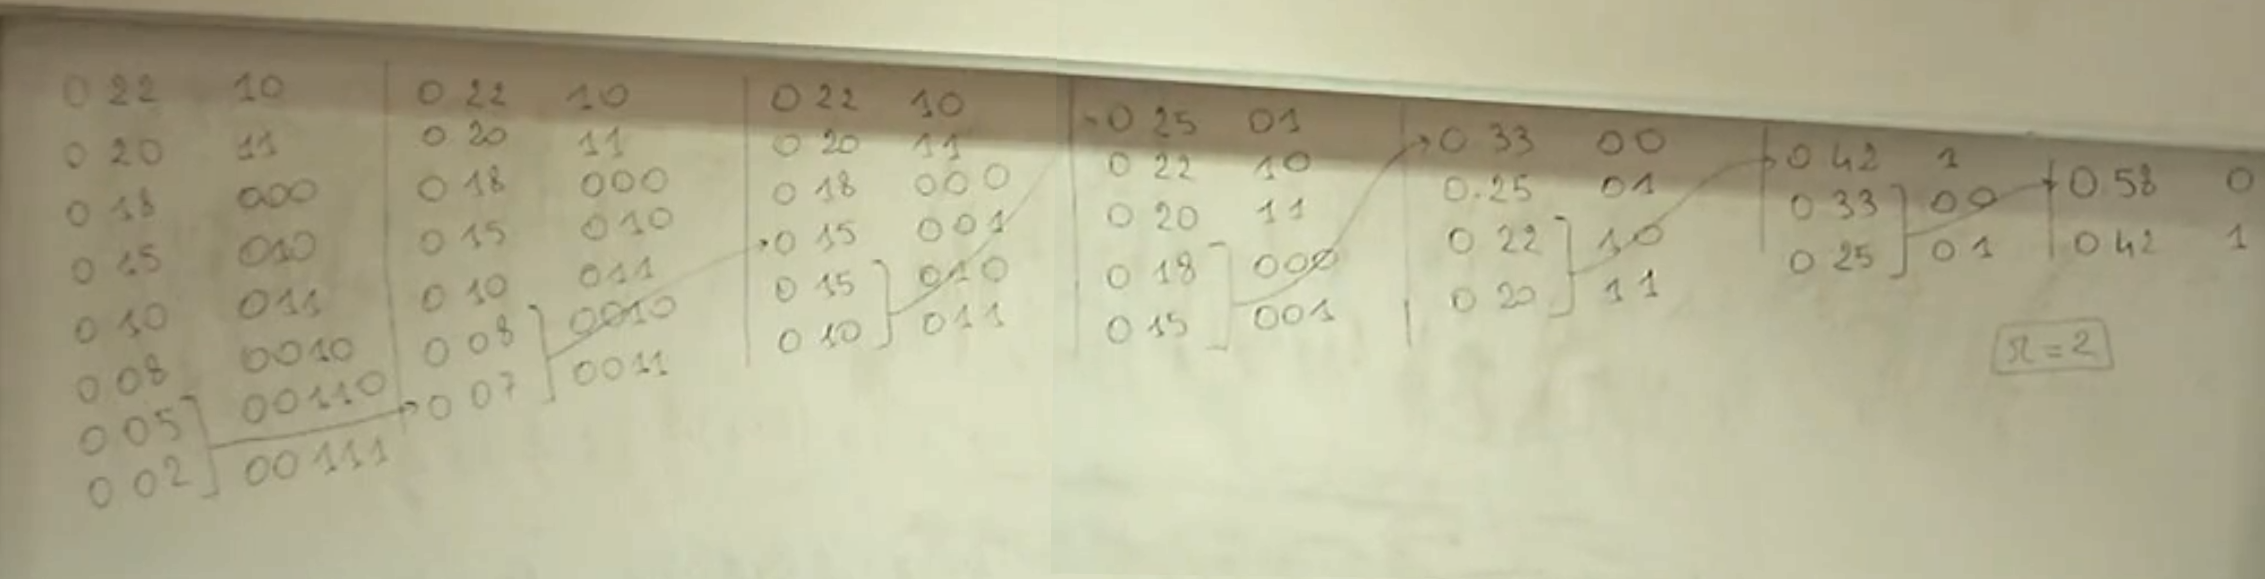
\includegraphics[width=\linewidth]{immagini/img22}
\end{figure}

\begin{equation*}
L_{binario} = 0.42 \cdot 2 + 0.43 \cdot 3 + 0.08 \cdot 4 + 0.07 \cdot 4 =
\end{equation*}
\begin{equation*}
= 0.84 + 1.29 + 0.32 + 0.35 = 2.13 + 0.67 = 2.8\; \frac{\text{bit}}{\text{simbolo}}
\end{equation*}

Mentre per $r=4$:

\begin{equation*}
L_{quattro} = 0.60 \cdot 1 + 0.33 \cdot 2 + 0.07 \cdot 3  =
\end{equation*}
\begin{equation*}
= 0.60 + 0.66 + 0.21 = 1.26 + 0.21 = 1.47\; \frac{\text{cifre quaternarie}}{\text{simbolo}}
\end{equation*}

Effettivamente potremmo passare da un codice all'altro utilizzando una tabella per la conversione dei codici:
\begin{table}[h]
	\centering
	\begin{tabular}{l|l}
		$\Gamma$ & binario \\
		\hline
		0        & 00      \\
		1        & 01      \\
		2        & 10      \\
		3        & 11     
	\end{tabular}
\end{table}

\begin{multicols}{2}
	\begin{center}
		$p_1=0.22 \rightarrow \texttt{1}$\\
		$p_2=0.20 \rightarrow \texttt{2}$\\
		$p_3=0.18 \rightarrow \texttt{3}$\\
		$p_4=0.15 \rightarrow \texttt{00}$\\
		$p_5=0.10 \rightarrow \texttt{01}$\\
		$p_6=0.08 \rightarrow \texttt{02}$\\
		$p_7=0.05 \rightarrow \texttt{030}$\\
		$p_8=0.02 \rightarrow \texttt{031}$\\
	\end{center}

\columnbreak

\begin{center}
	$p_1=0.22 \rightarrow \texttt{01}$\\
	$p_2=0.20 \rightarrow \texttt{11}$\\
	$p_3=0.18 \rightarrow \texttt{11}$\\
	$p_4=0.15 \rightarrow \texttt{0000}$\\
	$p_5=0.10 \rightarrow \texttt{0001}$\\
	$p_6=0.08 \rightarrow \texttt{0010}$\\
	$p_7=0.05 \rightarrow \texttt{001100}$\\
	$p_8=0.02 \rightarrow \texttt{001101}$\\
\end{center}
\end{multicols}

E viene un codice diverso da quello calcolato prima, la lunghezza media sarà il doppio di quella precedente (ogni simbolo di $\Sigma$ viene convertito in due simboli binari), quindi avrò che $L = 2 \cdot 1.47 = 2.94 \; \frac{\text{bit}}{\text{simbolo}}$, che è maggiore di $2.8 \; \frac{\text{bit}}{\text{simbolo}}$ calcolato applicando Huffman con $r=2$.\\
Possiamo quindi affermare che questo tipo di "scorciatoia" non produce un codice ottimale.

Come si dimostra che il codice prodotto sia ottimale (con $r=4$)? Allo stesso modo, si individuano le $r$ codeword più piccole e le si raggruppano ottenendo un albero $r$-ario (aggiungendo il giusto numero di simboli fittizi).

\subsection*{Robustezza codici di Huffman}
\addcontentsline{toc}{subsection}{Robustezza codici di Huffman}
Come mai si preferiscono codici con meno varianza (quindi a parità di probabilità metto il simbolo virtuale sopra)?

Data una sorgente $S$ noi stimiamo le probabilità di uscita dei simboli $s_i$ osservando in un lasso di tempo più o meno lungo.
In pratica calcolo dei $p_i'$ che sarebbero delle $p_i$ sommate ad un errore.
Ovviamente deve valere che 
\begin{equation*}
\sum_{i=1}^qp_i'=1
\end{equation*}
Ma dato che $p_i'=p_i+e_i$:
\begin{equation*}
\sum_{i=1}^qp_i'= \sum_{i=1}^qp_i + \sum_{i=1}^qe_i = 1
\end{equation*}
Quindi
\begin{equation*}
1=1 + \sum_{i=1}^qe_i
\end{equation*}
\begin{equation}
\sum_{i=1}^qe_i = 0 
\end{equation}
Quindi gli errori in media si "compensano" a vicenda (la coperta è corta: se la tiro da una parte si scopre l'altra ;))
La media degli errori è uguale a 0:
\begin{equation}
\frac{1}{q}\sum_{i=1}^qe_i = 0 
\end{equation}


La varianza di questi errori vale:

\begin{equation}
\sigma^2 = \frac{1}{q}\sum_{i=1}^qe_i^2
\end{equation}

E la lunghezza calcolata con le probabilità stimate?

\begin{equation*}
L'= \sum_{i=1}^qp_i'\ell_i = \sum_{i=1}^qp_i\ell_i + \sum_{i=1}^qe_i\ell_I = L + \sum_{i=1}^qe_i\ell_i
\end{equation*}

Quindi l'obiettivo è quello di minimizzare $\sum_{i=1}^qe_i\ell_i$.
Consideriamola come una funzione $f$ di $q$ variabili:

\begin{equation*}
min f(e_1, e_2, ... , e_q) = \sum_{i=1}^qe_i\ell_i
\end{equation*}
\begin{equation*}
\text{t.c.} \sum_{i=1}^qe_i\ell_i = 0 \; \; \; \; \; \;\land 
\end{equation*}
\begin{equation*}
\frac{1}{q} \sum_{i=1}^qe_i^2-\sigma^2 = 0
\end{equation*}
Per risolvere questo problema di minimo vincolato si usano i moltiplicatori di Lagrange:
\begin{equation*}
\mathscr{L}(l_1, ... ,l_q) = \sum_{i=1}^qe_i\ell_i - \lambda \sum_{i=1}^qe_i - \mu (\frac{1}{q}\sum_{i=1}^qe_i^2-\sigma^2)
\end{equation*}

Per risolvere questo problema uso le derivate:

\begin{equation*}
\frac{\partial \mathscr{L}}{\partial e_i} = \ell_i - \lambda - \frac{2\mu}{q}e_i = 0 \; \; \; \; \; \; \; \; \; \forall i \in \{1, 2, ..., q\}
\end{equation*}

Derivo rispetto a $\mathscr{L}$:
\begin{equation*}
\sum_{i=1}^q\ell_i-\lambda q - \frac{2\mu}{q}\sum_{i=1}^qe_i = 0
\end{equation*}
Ma ricordiamo che $\sum_{i=1}^qe_i = 0$, quindi
\begin{empheq}[box=\tcbhighmath]{equation*}
\lambda = \frac{1}{q} \sum_{i=1}^q\ell_i
\end{empheq}

Derivo rispetto a $e_i$:
\begin{equation*}
\sum_{i=1}^qe_i\ell_i-\lambda \sum_{i=1}^qe_i - \frac{2\mu}{q}\sum_{i=1}^qe_i^2 = 0
\end{equation*}
Ma ricordiamo che $\sum_{i=1}^qe_i = 0$ e che $\frac{1}{q}\sum_{i=1}^qe_i^2 = 0$, quindi
\begin{equation*}
\sum_{i=1}^q\ell_i - 2\mu \sigma^2 = 0
\end{equation*}
\begin{empheq}[box=\tcbhighmath]{equation*}
\mu = \frac{1}{2\sigma^2}\sum_{i=1}^qe_i\ell_i
\end{empheq}

Ora sostituiamo i moltiplicatori appena trovati all'interno di 
\begin{equation*}
\frac{\partial \mathscr{L}}{\partial e_i} = \ell_i - \lambda - \frac{2\mu}{q}e_i = 0
\end{equation*}
e otterremo:
\begin{equation*}
\sum_{i=1}^q\ell_i^2 - \frac{1}{q}(\sum_{i=1}^q\ell_i)^2-\frac{1}{q\sigma^2}(\sum_{i=1}^qe_i\ell_i)^2 = 0
\end{equation*}
\begin{equation*}
(\sum_{i=1}^qe_i\ell_i)^2 = \sigma^2[q\sum_{i=1}^q\ell_i - (\sum_{i=1}^q\ell_i)^2]
\end{equation*}
\begin{equation*}
\sigma^2q^2[\frac{1}{q}\sum_{i=1}^q\ell_i^2-(\frac{1}{q}\sum_{i=1}^q\ell-_i)^2]
\end{equation*}
\begin{equation*}
= \sigma^2q^2[var(\ell_i)]
\end{equation*}

Quindi otteniamo che la quantità che vogliamo minimizzare è proporzionale alla varianza delle $\ell_i$ moltiplicata per il numero di simboli della sorgente al quadrato e il quadrato di sigma.
Quindi più piccola è la varianza di $\ell_i$ più è piccola la sommatoria degli errori che vogliamo minimizzare (che rappresenta l'errore con cui conosco le probabilità $p_i'$).\\
Quindi varianza minore rappresenta una minor differenza $L - L'$.
In questo modo rendiamo 'robusto' il codice di Huffman: rendiamo la lunghezza media meno sensibile agli errori.
All'orale interessano i concetti, non saper rifare tutto il calcolo (però sapere il procedimento e le conclusioni)